På de neste oppgavene bruker vi funksjonsgeneratoren TG550 som signalkilde.
Vi stiller inn funksjonsgeneratoren og oscilloskopet slik det er
beskrevet i oppgaven.

\subsection{Oppg 3}
A settes til 5 volt.  
Inngangssignalet til B er en sinusspenning med frekvens 1 kHz og vi varier
signalamplituden (Vpp) fra 2 til 6 Vpp. 
Vi sammenligner inngangssignal og utgangssignal.
\\\\
For input Vpp fra 2V og oppover får vi utslag i output signalet.
Der hvor input signalet er over 2V får vi en negativ puls på output.
\begin{figure}[!ht]
  \caption{Sinusfunksjon på input B og output-signal.}
  \centering
    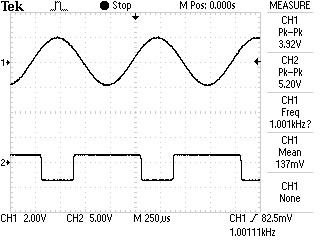
\includegraphics[width=\textwidth]{3.jpg}
\end{figure}
